\subsection{享元模式(Flyweight)}

\subsubsection{享元模式简介}

享元模式是一种常用的设计模式。它通过共享来有效地支持大量细粒度的对象。享元模式通过共享内部状态来减少内存的使用,并用不同的外部状态来区分不同的对象。这样可以在不需要额外内存的情况下创建大量的对象。

例如,在游戏中,可能会有大量的敌人。如果每个敌人都是一个单独的对象,将会消耗大量的内存。如果使用享元模式,可以将所有敌人都共享一个基础对象,并使用不同的外部状态来区分不同的敌人。这样就可以在不需要额外内存的情况下创建大量敌人。

\subsubsection{享元模式在项目中的应用}

\begin{figure}[H]
  \centering
  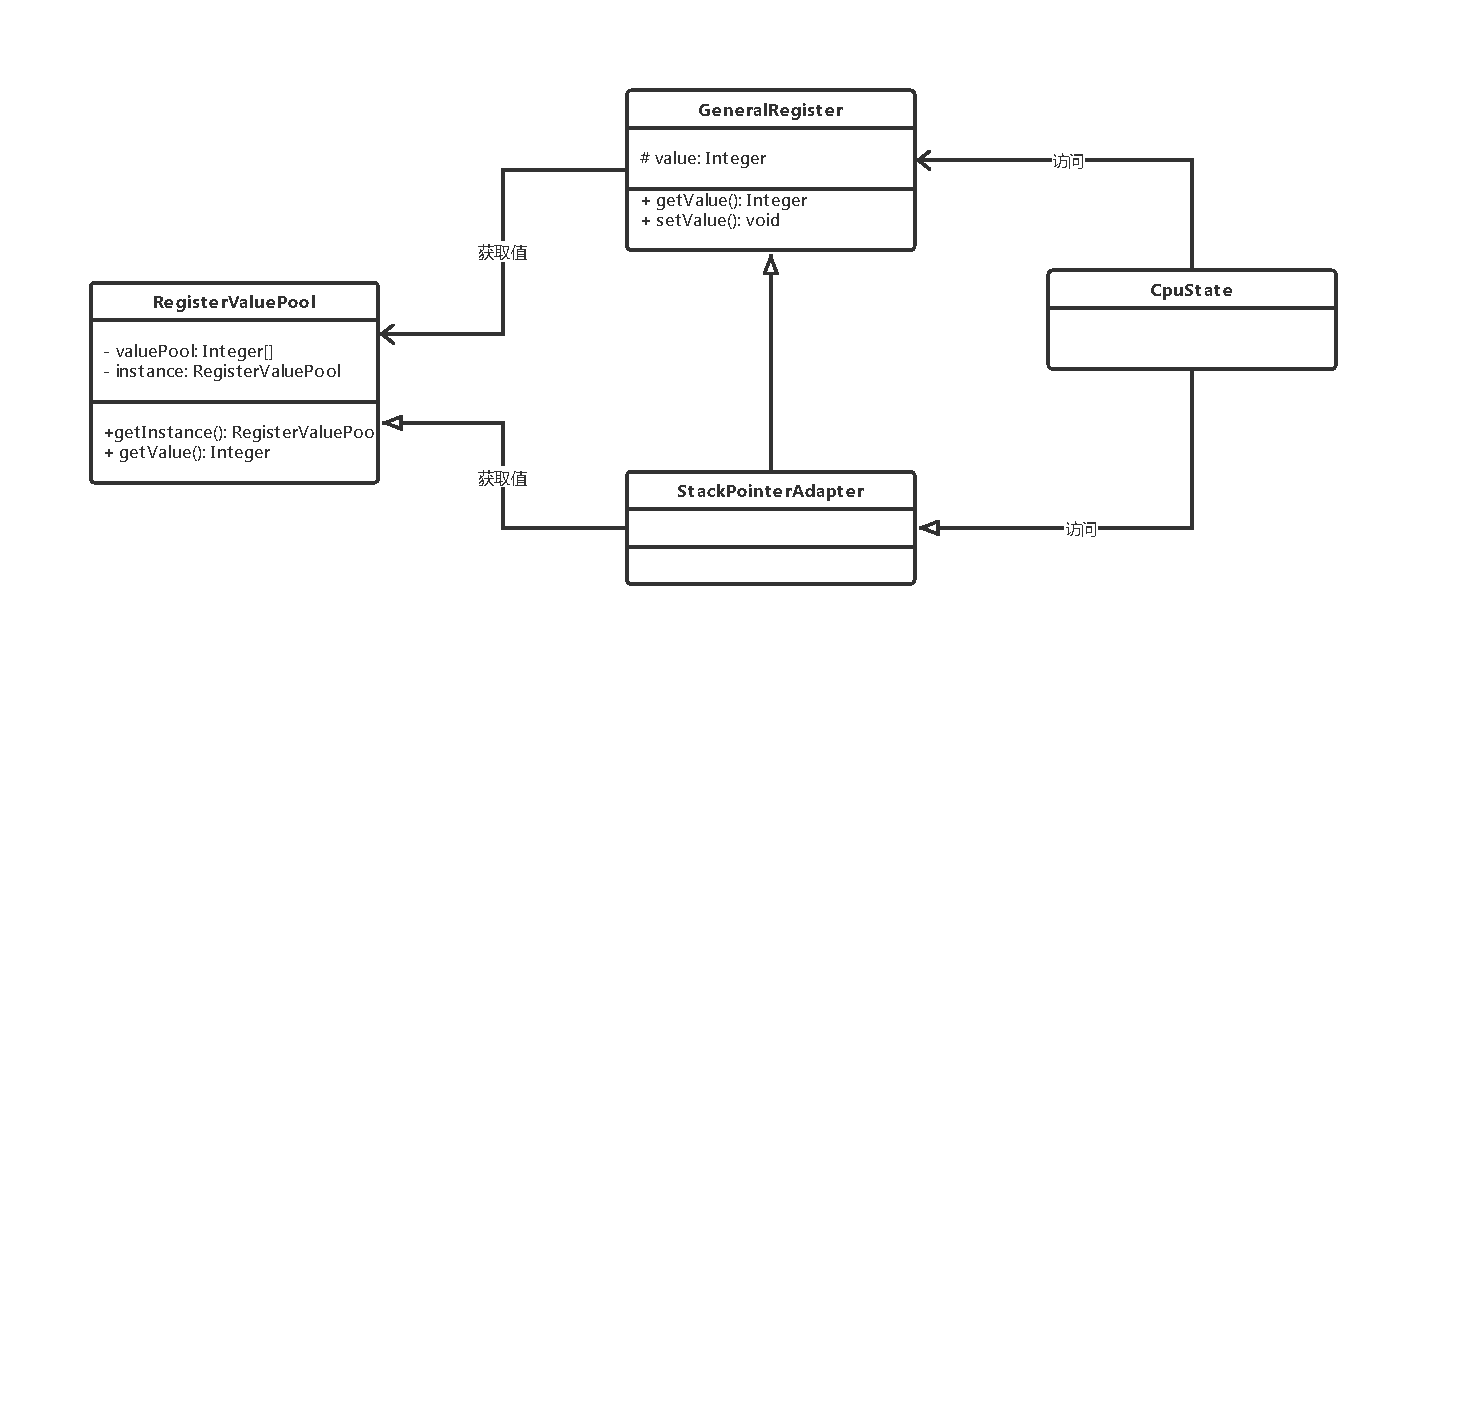
\includegraphics[width=0.9\textwidth]{figures/享元模式.pdf}
  \caption{享元模式在 Slow6502 中的类图}
\end{figure}

在我们的项目中,享元模式被应用在管理寄存器的值这个任务上。享元模式在这种情况下可以帮助减少内存的使用。寄存器通常都是固定大小的,因此使用享元模式可以让我们创建大量的寄存器,而不需要为每个寄存器单独分配内存。相反,我们可以共享一个基础对象来管理寄存器的值,并用不同的外部状态来区分不同的寄存器。

另外,使用享元模式还可以提高程序的性能。对于大量细粒度的对象,每个对象都需要单独分配内存和维护其状态。这样会消耗大量的 CPU 时间和内存空间。通过使用享元模式,可以减少内存分配和状态维护的开销,从而提高程序的性能。
